\documentclass[]{article}
\usepackage{lmodern}
\usepackage{amssymb,amsmath}
\usepackage{ifxetex,ifluatex}
\usepackage{fixltx2e} % provides \textsubscript
\ifnum 0\ifxetex 1\fi\ifluatex 1\fi=0 % if pdftex
  \usepackage[T1]{fontenc}
  \usepackage[utf8]{inputenc}
\else % if luatex or xelatex
  \ifxetex
    \usepackage{mathspec}
  \else
    \usepackage{fontspec}
  \fi
  \defaultfontfeatures{Ligatures=TeX,Scale=MatchLowercase}
\fi
% use upquote if available, for straight quotes in verbatim environments
\IfFileExists{upquote.sty}{\usepackage{upquote}}{}
% use microtype if available
\IfFileExists{microtype.sty}{%
\usepackage{microtype}
\UseMicrotypeSet[protrusion]{basicmath} % disable protrusion for tt fonts
}{}
\usepackage[margin=2.54cm]{geometry}
\usepackage{hyperref}
\hypersetup{unicode=true,
            pdftitle={Assignment 8: Mapping},
            pdfauthor={Jake Greif},
            pdfborder={0 0 0},
            breaklinks=true}
\urlstyle{same}  % don't use monospace font for urls
\usepackage{color}
\usepackage{fancyvrb}
\newcommand{\VerbBar}{|}
\newcommand{\VERB}{\Verb[commandchars=\\\{\}]}
\DefineVerbatimEnvironment{Highlighting}{Verbatim}{commandchars=\\\{\}}
% Add ',fontsize=\small' for more characters per line
\usepackage{framed}
\definecolor{shadecolor}{RGB}{248,248,248}
\newenvironment{Shaded}{\begin{snugshade}}{\end{snugshade}}
\newcommand{\AlertTok}[1]{\textcolor[rgb]{0.94,0.16,0.16}{#1}}
\newcommand{\AnnotationTok}[1]{\textcolor[rgb]{0.56,0.35,0.01}{\textbf{\textit{#1}}}}
\newcommand{\AttributeTok}[1]{\textcolor[rgb]{0.77,0.63,0.00}{#1}}
\newcommand{\BaseNTok}[1]{\textcolor[rgb]{0.00,0.00,0.81}{#1}}
\newcommand{\BuiltInTok}[1]{#1}
\newcommand{\CharTok}[1]{\textcolor[rgb]{0.31,0.60,0.02}{#1}}
\newcommand{\CommentTok}[1]{\textcolor[rgb]{0.56,0.35,0.01}{\textit{#1}}}
\newcommand{\CommentVarTok}[1]{\textcolor[rgb]{0.56,0.35,0.01}{\textbf{\textit{#1}}}}
\newcommand{\ConstantTok}[1]{\textcolor[rgb]{0.00,0.00,0.00}{#1}}
\newcommand{\ControlFlowTok}[1]{\textcolor[rgb]{0.13,0.29,0.53}{\textbf{#1}}}
\newcommand{\DataTypeTok}[1]{\textcolor[rgb]{0.13,0.29,0.53}{#1}}
\newcommand{\DecValTok}[1]{\textcolor[rgb]{0.00,0.00,0.81}{#1}}
\newcommand{\DocumentationTok}[1]{\textcolor[rgb]{0.56,0.35,0.01}{\textbf{\textit{#1}}}}
\newcommand{\ErrorTok}[1]{\textcolor[rgb]{0.64,0.00,0.00}{\textbf{#1}}}
\newcommand{\ExtensionTok}[1]{#1}
\newcommand{\FloatTok}[1]{\textcolor[rgb]{0.00,0.00,0.81}{#1}}
\newcommand{\FunctionTok}[1]{\textcolor[rgb]{0.00,0.00,0.00}{#1}}
\newcommand{\ImportTok}[1]{#1}
\newcommand{\InformationTok}[1]{\textcolor[rgb]{0.56,0.35,0.01}{\textbf{\textit{#1}}}}
\newcommand{\KeywordTok}[1]{\textcolor[rgb]{0.13,0.29,0.53}{\textbf{#1}}}
\newcommand{\NormalTok}[1]{#1}
\newcommand{\OperatorTok}[1]{\textcolor[rgb]{0.81,0.36,0.00}{\textbf{#1}}}
\newcommand{\OtherTok}[1]{\textcolor[rgb]{0.56,0.35,0.01}{#1}}
\newcommand{\PreprocessorTok}[1]{\textcolor[rgb]{0.56,0.35,0.01}{\textit{#1}}}
\newcommand{\RegionMarkerTok}[1]{#1}
\newcommand{\SpecialCharTok}[1]{\textcolor[rgb]{0.00,0.00,0.00}{#1}}
\newcommand{\SpecialStringTok}[1]{\textcolor[rgb]{0.31,0.60,0.02}{#1}}
\newcommand{\StringTok}[1]{\textcolor[rgb]{0.31,0.60,0.02}{#1}}
\newcommand{\VariableTok}[1]{\textcolor[rgb]{0.00,0.00,0.00}{#1}}
\newcommand{\VerbatimStringTok}[1]{\textcolor[rgb]{0.31,0.60,0.02}{#1}}
\newcommand{\WarningTok}[1]{\textcolor[rgb]{0.56,0.35,0.01}{\textbf{\textit{#1}}}}
\usepackage{graphicx,grffile}
\makeatletter
\def\maxwidth{\ifdim\Gin@nat@width>\linewidth\linewidth\else\Gin@nat@width\fi}
\def\maxheight{\ifdim\Gin@nat@height>\textheight\textheight\else\Gin@nat@height\fi}
\makeatother
% Scale images if necessary, so that they will not overflow the page
% margins by default, and it is still possible to overwrite the defaults
% using explicit options in \includegraphics[width, height, ...]{}
\setkeys{Gin}{width=\maxwidth,height=\maxheight,keepaspectratio}
\IfFileExists{parskip.sty}{%
\usepackage{parskip}
}{% else
\setlength{\parindent}{0pt}
\setlength{\parskip}{6pt plus 2pt minus 1pt}
}
\setlength{\emergencystretch}{3em}  % prevent overfull lines
\providecommand{\tightlist}{%
  \setlength{\itemsep}{0pt}\setlength{\parskip}{0pt}}
\setcounter{secnumdepth}{0}
% Redefines (sub)paragraphs to behave more like sections
\ifx\paragraph\undefined\else
\let\oldparagraph\paragraph
\renewcommand{\paragraph}[1]{\oldparagraph{#1}\mbox{}}
\fi
\ifx\subparagraph\undefined\else
\let\oldsubparagraph\subparagraph
\renewcommand{\subparagraph}[1]{\oldsubparagraph{#1}\mbox{}}
\fi

%%% Use protect on footnotes to avoid problems with footnotes in titles
\let\rmarkdownfootnote\footnote%
\def\footnote{\protect\rmarkdownfootnote}

%%% Change title format to be more compact
\usepackage{titling}

% Create subtitle command for use in maketitle
\providecommand{\subtitle}[1]{
  \posttitle{
    \begin{center}\large#1\end{center}
    }
}

\setlength{\droptitle}{-2em}

  \title{Assignment 8: Mapping}
    \pretitle{\vspace{\droptitle}\centering\huge}
  \posttitle{\par}
    \author{Jake Greif}
    \preauthor{\centering\large\emph}
  \postauthor{\par}
    \date{}
    \predate{}\postdate{}
  

\begin{document}
\maketitle

\hypertarget{overview}{%
\subsection{OVERVIEW}\label{overview}}

This exercise accompanies the lessons in Hydrologic Data Analysis on
mapping

\hypertarget{directions}{%
\subsection{Directions}\label{directions}}

\begin{enumerate}
\def\labelenumi{\arabic{enumi}.}
\tightlist
\item
  Change ``Student Name'' on line 3 (above) with your name.
\item
  Work through the steps, \textbf{creating code and output} that fulfill
  each instruction.
\item
  Be sure to \textbf{answer the questions} in this assignment document.
\item
  When you have completed the assignment, \textbf{Knit} the text and
  code into a single pdf file.
\item
  After Knitting, submit the completed exercise (pdf file) to the
  dropbox in Sakai. Add your last name into the file name (e.g.,
  ``A08\_Salk.html'') prior to submission.
\end{enumerate}

The completed exercise is due on 23 October 2019 at 9:00 am.

\hypertarget{setup}{%
\subsection{Setup}\label{setup}}

\begin{enumerate}
\def\labelenumi{\arabic{enumi}.}
\tightlist
\item
  Verify your working directory is set to the R project file,
\item
  Load the tidyverse, lubridate, cowplot, LAGOSNE, sf, maps, and viridis
  packages.
\item
  Set your ggplot theme (can be theme\_classic or something else)
\item
  Load the lagos database, the USA rivers water features shape file, and
  the HUC6 watershed shape file.
\end{enumerate}

\begin{Shaded}
\begin{Highlighting}[]
\KeywordTok{getwd}\NormalTok{()}
\end{Highlighting}
\end{Shaded}

\begin{verbatim}
## [1] "/Users/jakegreif/Duke/Fall_2019/Hydrologic_Data_Analysis"
\end{verbatim}

\begin{Shaded}
\begin{Highlighting}[]
\KeywordTok{library}\NormalTok{(tidyverse)}
\end{Highlighting}
\end{Shaded}

\begin{verbatim}
## -- Attaching packages ------------------------------------------------------------------------ tidyverse 1.2.1 --
\end{verbatim}

\begin{verbatim}
## v ggplot2 3.2.1     v purrr   0.3.2
## v tibble  2.1.3     v dplyr   0.8.3
## v tidyr   1.0.0     v stringr 1.4.0
## v readr   1.3.1     v forcats 0.4.0
\end{verbatim}

\begin{verbatim}
## -- Conflicts --------------------------------------------------------------------------- tidyverse_conflicts() --
## x dplyr::filter() masks stats::filter()
## x dplyr::lag()    masks stats::lag()
\end{verbatim}

\begin{Shaded}
\begin{Highlighting}[]
\KeywordTok{library}\NormalTok{(lubridate)}
\end{Highlighting}
\end{Shaded}

\begin{verbatim}
## 
## Attaching package: 'lubridate'
\end{verbatim}

\begin{verbatim}
## The following object is masked from 'package:base':
## 
##     date
\end{verbatim}

\begin{Shaded}
\begin{Highlighting}[]
\KeywordTok{library}\NormalTok{(cowplot)}
\end{Highlighting}
\end{Shaded}

\begin{verbatim}
## 
## ********************************************************
\end{verbatim}

\begin{verbatim}
## Note: As of version 1.0.0, cowplot does not change the
\end{verbatim}

\begin{verbatim}
##   default ggplot2 theme anymore. To recover the previous
\end{verbatim}

\begin{verbatim}
##   behavior, execute:
##   theme_set(theme_cowplot())
\end{verbatim}

\begin{verbatim}
## ********************************************************
\end{verbatim}

\begin{verbatim}
## 
## Attaching package: 'cowplot'
\end{verbatim}

\begin{verbatim}
## The following object is masked from 'package:lubridate':
## 
##     stamp
\end{verbatim}

\begin{Shaded}
\begin{Highlighting}[]
\KeywordTok{library}\NormalTok{(LAGOSNE)}
\KeywordTok{library}\NormalTok{(sf)}
\end{Highlighting}
\end{Shaded}

\begin{verbatim}
## Linking to GEOS 3.7.2, GDAL 2.4.2, PROJ 5.2.0
\end{verbatim}

\begin{Shaded}
\begin{Highlighting}[]
\KeywordTok{library}\NormalTok{(maps)}
\end{Highlighting}
\end{Shaded}

\begin{verbatim}
## 
## Attaching package: 'maps'
\end{verbatim}

\begin{verbatim}
## The following object is masked from 'package:purrr':
## 
##     map
\end{verbatim}

\begin{Shaded}
\begin{Highlighting}[]
\KeywordTok{library}\NormalTok{(viridis)}
\end{Highlighting}
\end{Shaded}

\begin{verbatim}
## Loading required package: viridisLite
\end{verbatim}

\begin{Shaded}
\begin{Highlighting}[]
\KeywordTok{theme_set}\NormalTok{(}\KeywordTok{theme_classic}\NormalTok{())}

\NormalTok{LAGOSdata <-}\StringTok{ }\KeywordTok{lagosne_load}\NormalTok{()}
\end{Highlighting}
\end{Shaded}

\begin{verbatim}
## Warning in `_f`(version = version, fpath = fpath): LAGOSNE version
## unspecified, loading version: 1.087.3
\end{verbatim}

\begin{Shaded}
\begin{Highlighting}[]
\NormalTok{waterfeatures <-}\StringTok{ }\KeywordTok{st_read}\NormalTok{(}\StringTok{"./Data/Raw/hydrogl020.dbf"}\NormalTok{)}
\end{Highlighting}
\end{Shaded}

\begin{verbatim}
## Reading layer `hydrogl020' from data source `/Users/jakegreif/Duke/Fall_2019/Hydrologic_Data_Analysis/Data/Raw/hydrogl020.dbf' using driver `ESRI Shapefile'
## Simple feature collection with 76975 features and 12 fields
## geometry type:  LINESTRING
## dimension:      XY
## bbox:           xmin: -179.9982 ymin: 17.67469 xmax: 179.9831 ymax: 71.39819
## epsg (SRID):    NA
## proj4string:    NA
\end{verbatim}

\begin{Shaded}
\begin{Highlighting}[]
\NormalTok{HUC6 <-}\StringTok{ }\KeywordTok{st_read}\NormalTok{(}\StringTok{"./Data/Raw/Watersheds_Spatial/WBDHU6.dbf"}\NormalTok{)}
\end{Highlighting}
\end{Shaded}

\begin{verbatim}
## Reading layer `WBDHU6' from data source `/Users/jakegreif/Duke/Fall_2019/Hydrologic_Data_Analysis/Data/Raw/Watersheds_Spatial/WBDHU6.dbf' using driver `ESRI Shapefile'
## Simple feature collection with 33 features and 15 fields
## geometry type:  MULTIPOLYGON
## dimension:      XY
## bbox:           xmin: -90.6235 ymin: 24.39533 xmax: -75.3981 ymax: 37.52103
## epsg (SRID):    4269
## proj4string:    +proj=longlat +ellps=GRS80 +towgs84=0,0,0,0,0,0,0 +no_defs
\end{verbatim}

\hypertarget{mapping-water-quality-in-lakes}{%
\subsection{Mapping water quality in
lakes}\label{mapping-water-quality-in-lakes}}

Complete the in-class exercise from lesson 15, to map average secchi
depth measurements across states in Maine, considering lake area and
lake depth as predictors for water clarity. Steps here are identical to
the lesson, with the following edits:

\begin{itemize}
\tightlist
\item
  Make sure all your wrangling is done in this document (this includes
  basic wrangling of the LAGOS database)
\item
  In your cowplot, do not adjust the legend items (even though they look
  ugly). Rather, reflect on how you would improve them with additional
  coding.
\item
  For item 9, \textbf{do} run a regression on secchi depth by lake area
  and a separate regression on secchi depth by lake depth. Make
  scatterplots of these relationships. Note that log-transforming one of
  these items may be necessary.
\end{itemize}

\begin{enumerate}
\def\labelenumi{\arabic{enumi}.}
\setcounter{enumi}{4}
\tightlist
\item
  Filter the states and secchi depth datasets so that they contain Maine
  only. For the secchi depth dataset, create a summary dataset with just
  the mean secchi depth.
\end{enumerate}

\begin{Shaded}
\begin{Highlighting}[]
\CommentTok{# load LAGOSNE data frames}
\NormalTok{LAGOSlocus <-}\StringTok{ }\NormalTok{LAGOSdata}\OperatorTok{$}\NormalTok{locus}
\NormalTok{LAGOSstate <-}\StringTok{ }\NormalTok{LAGOSdata}\OperatorTok{$}\NormalTok{state}
\NormalTok{LAGOSnutrient <-}\StringTok{ }\NormalTok{LAGOSdata}\OperatorTok{$}\NormalTok{epi_nutr}
\NormalTok{LAGOSlimno <-}\StringTok{ }\NormalTok{LAGOSdata}\OperatorTok{$}\NormalTok{lakes_limno}

\CommentTok{# Create a data frame to visualize secchi depth}
\NormalTok{LAGOScombined <-}\StringTok{ }
\StringTok{  }\KeywordTok{left_join}\NormalTok{(LAGOSnutrient, LAGOSlocus) }\OperatorTok
\StringTok{  }\KeywordTok{left_join}\NormalTok{(., LAGOSlimno) }\OperatorTok
\StringTok{  }\KeywordTok{left_join}\NormalTok{(., LAGOSstate) }\OperatorTok
\StringTok{  }\KeywordTok{filter}\NormalTok{(}\OperatorTok{!}\KeywordTok{is.na}\NormalTok{(state)) }\OperatorTok
\StringTok{  }\KeywordTok{select}\NormalTok{(lagoslakeid, sampledate, secchi, lake_area_ha,}
\NormalTok{         maxdepth, nhd_lat, nhd_long, state)}
\end{Highlighting}
\end{Shaded}

\begin{verbatim}
## Joining, by = "lagoslakeid"
\end{verbatim}

\begin{verbatim}
## Joining, by = c("lagoslakeid", "nhdid", "nhd_lat", "nhd_long")
\end{verbatim}

\begin{verbatim}
## Joining, by = "state_zoneid"
\end{verbatim}

\begin{Shaded}
\begin{Highlighting}[]
\CommentTok{# Isolate Maine data}
\NormalTok{states <-}\StringTok{ }\KeywordTok{st_as_sf}\NormalTok{(}\KeywordTok{map}\NormalTok{(}\DataTypeTok{database =} \StringTok{"state"}\NormalTok{, }\DataTypeTok{plot =} \OtherTok{TRUE}\NormalTok{, }
                       \DataTypeTok{fill =} \OtherTok{TRUE}\NormalTok{, }\DataTypeTok{col =} \StringTok{"white"}\NormalTok{))}
\end{Highlighting}
\end{Shaded}

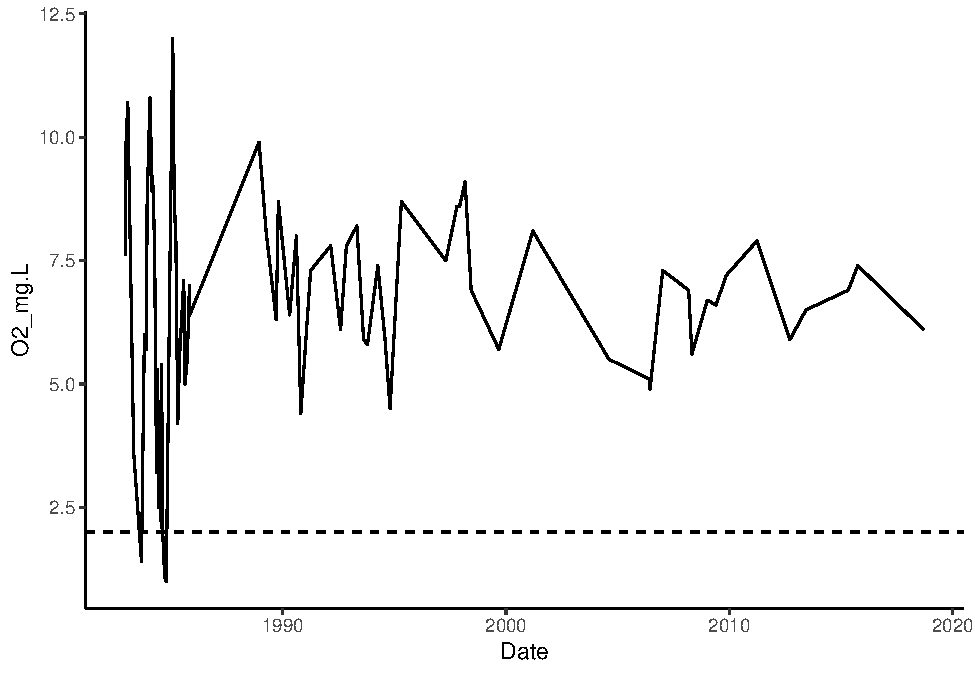
\includegraphics{A08_Mapping_files/figure-latex/unnamed-chunk-1-1.pdf}

\begin{Shaded}
\begin{Highlighting}[]
\NormalTok{Maine <-}\StringTok{ }\KeywordTok{filter}\NormalTok{(states, ID }\OperatorTok{==}\StringTok{ "maine"}\NormalTok{)}

\NormalTok{Maine.dat <-}\StringTok{ }\KeywordTok{filter}\NormalTok{(LAGOScombined, state }\OperatorTok{==}\StringTok{ "ME"}\NormalTok{) }\OperatorTok
\StringTok{  }\KeywordTok{group_by}\NormalTok{(lagoslakeid) }\OperatorTok
\StringTok{  }\KeywordTok{summarise}\NormalTok{(}\DataTypeTok{secchi.mean =} \KeywordTok{mean}\NormalTok{(secchi),}
            \DataTypeTok{area =} \KeywordTok{mean}\NormalTok{(lake_area_ha),}
            \DataTypeTok{depth =} \KeywordTok{mean}\NormalTok{(maxdepth),}
            \DataTypeTok{lat =} \KeywordTok{mean}\NormalTok{(nhd_lat), }
            \DataTypeTok{long =} \KeywordTok{mean}\NormalTok{(nhd_long)) }\OperatorTok
\StringTok{  }\KeywordTok{drop_na}\NormalTok{()}

\NormalTok{Maine.spatial <-}\StringTok{ }\KeywordTok{st_as_sf}\NormalTok{(Maine.dat, }\DataTypeTok{coords =} \KeywordTok{c}\NormalTok{(}\StringTok{"long"}\NormalTok{, }\StringTok{"lat"}\NormalTok{), }\DataTypeTok{crs =} \DecValTok{4326}\NormalTok{)}
\end{Highlighting}
\end{Shaded}

\begin{enumerate}
\def\labelenumi{\arabic{enumi}.}
\setcounter{enumi}{5}
\tightlist
\item
  Create a plot of mean secchi depth for lakes in Maine, with mean
  secchi depth designated as color and the lake area as the size of the
  dot. Remember that you are using size in the aesthetics and should
  remove the size = 1 from the other part of the code. Adjust the
  transparency of points as needed.
\end{enumerate}

\begin{Shaded}
\begin{Highlighting}[]
\NormalTok{Maine.plot <-}\StringTok{ }\KeywordTok{ggplot}\NormalTok{() }\OperatorTok{+}
\StringTok{  }\KeywordTok{geom_sf}\NormalTok{(}\DataTypeTok{data =}\NormalTok{ Maine, }\DataTypeTok{fill =} \StringTok{"white"}\NormalTok{) }\OperatorTok{+}
\StringTok{  }\KeywordTok{geom_sf}\NormalTok{(}\DataTypeTok{data =}\NormalTok{ Maine.spatial, }\KeywordTok{aes}\NormalTok{(}\DataTypeTok{color =}\NormalTok{ secchi.mean, }\DataTypeTok{size =}\NormalTok{ area), }
          \DataTypeTok{alpha =} \FloatTok{0.5}\NormalTok{) }\OperatorTok{+}
\StringTok{  }\KeywordTok{scale_color_viridis_c}\NormalTok{() }\OperatorTok{+}
\StringTok{  }\KeywordTok{labs}\NormalTok{(}\DataTypeTok{color =} \StringTok{"Average Secchi Depth (m)"}\NormalTok{) }\OperatorTok{+}
\StringTok{  }\KeywordTok{theme}\NormalTok{(}\DataTypeTok{legend.position =} \StringTok{"top"}\NormalTok{)}
\KeywordTok{print}\NormalTok{(Maine.plot)}
\end{Highlighting}
\end{Shaded}

\includegraphics{A08_Mapping_files/figure-latex/unnamed-chunk-2-1.pdf}

\begin{enumerate}
\def\labelenumi{\arabic{enumi}.}
\setcounter{enumi}{6}
\tightlist
\item
  Create a second plot, but this time use maximum depth of the lake as
  the size of the dot.
\end{enumerate}

\begin{Shaded}
\begin{Highlighting}[]
\NormalTok{Maine.plot2 <-}\StringTok{ }\KeywordTok{ggplot}\NormalTok{() }\OperatorTok{+}
\StringTok{  }\KeywordTok{geom_sf}\NormalTok{(}\DataTypeTok{data =}\NormalTok{ Maine, }\DataTypeTok{fill =} \StringTok{"white"}\NormalTok{) }\OperatorTok{+}
\StringTok{  }\KeywordTok{geom_sf}\NormalTok{(}\DataTypeTok{data =}\NormalTok{ Maine.spatial, }\KeywordTok{aes}\NormalTok{(}\DataTypeTok{color =}\NormalTok{ secchi.mean, }\DataTypeTok{size =}\NormalTok{ depth), }
          \DataTypeTok{alpha =} \FloatTok{0.5}\NormalTok{) }\OperatorTok{+}
\StringTok{  }\KeywordTok{scale_color_viridis_c}\NormalTok{() }\OperatorTok{+}
\StringTok{  }\KeywordTok{labs}\NormalTok{(}\DataTypeTok{color =} \StringTok{"Average Secchi Depth (m)"}\NormalTok{) }\OperatorTok{+}
\StringTok{  }\KeywordTok{theme}\NormalTok{(}\DataTypeTok{legend.position =} \StringTok{"top"}\NormalTok{)}

\KeywordTok{print}\NormalTok{(Maine.plot2)}
\end{Highlighting}
\end{Shaded}

\includegraphics{A08_Mapping_files/figure-latex/unnamed-chunk-3-1.pdf}

\begin{enumerate}
\def\labelenumi{\arabic{enumi}.}
\setcounter{enumi}{7}
\tightlist
\item
  Plot these maps in the same plot with the \texttt{plot\_grid}
  function. Don't worry about adjusting the legends (if you have extra
  time this would be a good bonus task).
\end{enumerate}

\begin{Shaded}
\begin{Highlighting}[]
\KeywordTok{plot_grid}\NormalTok{(Maine.plot, Maine.plot2)}
\end{Highlighting}
\end{Shaded}

\includegraphics{A08_Mapping_files/figure-latex/unnamed-chunk-4-1.pdf}

What would you change about the legend to make it a more effective
visualization?

\begin{quote}
I would remove one of the Average secchi depth scales as well as both
the depth and lake size components of the legend. In order to
differentiate between the maps, I would include what the dot size
indicates in the title for each plot.
\end{quote}

\begin{enumerate}
\def\labelenumi{\arabic{enumi}.}
\setcounter{enumi}{8}
\tightlist
\item
  What relationships do you see between secchi depth, lake area, and
  lake depth? Which of the two lake variables seems to be a stronger
  determinant of secchi depth? (make a scatterplot and run a regression
  to test this)
\end{enumerate}

\emph{Note: consider log-transforming a predictor variable if
appropriate}

\begin{Shaded}
\begin{Highlighting}[]
\NormalTok{Maine.depth.plot <-}\StringTok{ }\KeywordTok{ggplot}\NormalTok{(Maine.dat, }\KeywordTok{aes}\NormalTok{(}\DataTypeTok{x =}\NormalTok{ secchi.mean, }\DataTypeTok{y =}\NormalTok{ depth)) }\OperatorTok{+}
\StringTok{  }\KeywordTok{geom_point}\NormalTok{() }\OperatorTok{+}
\StringTok{  }\KeywordTok{geom_smooth}\NormalTok{(}\DataTypeTok{method =} \StringTok{'lm'}\NormalTok{)}
\KeywordTok{print}\NormalTok{(Maine.depth.plot)}
\end{Highlighting}
\end{Shaded}

\includegraphics{A08_Mapping_files/figure-latex/unnamed-chunk-5-1.pdf}

\begin{Shaded}
\begin{Highlighting}[]
\NormalTok{Maine.depth.model <-}\StringTok{ }\KeywordTok{lm}\NormalTok{(}\DataTypeTok{data =}\NormalTok{ Maine.dat, depth }\OperatorTok{~}\StringTok{ }\NormalTok{secchi.mean)}
\KeywordTok{summary}\NormalTok{(Maine.depth.model)}
\end{Highlighting}
\end{Shaded}

\begin{verbatim}
## 
## Call:
## lm(formula = depth ~ secchi.mean, data = Maine.dat)
## 
## Residuals:
##     Min      1Q  Median      3Q     Max 
## -25.971  -4.605  -1.679   2.311  41.476 
## 
## Coefficients:
##             Estimate Std. Error t value Pr(>|t|)    
## (Intercept)  -0.6005     0.7671  -0.783    0.434    
## secchi.mean   2.8548     0.1524  18.738   <2e-16 ***
## ---
## Signif. codes:  0 '***' 0.001 '**' 0.01 '*' 0.05 '.' 0.1 ' ' 1
## 
## Residual standard error: 7.784 on 547 degrees of freedom
## Multiple R-squared:  0.3909, Adjusted R-squared:  0.3898 
## F-statistic: 351.1 on 1 and 547 DF,  p-value: < 2.2e-16
\end{verbatim}

\begin{Shaded}
\begin{Highlighting}[]
\NormalTok{Maine.area.plot <-}\StringTok{ }\KeywordTok{ggplot}\NormalTok{(Maine.dat, }\KeywordTok{aes}\NormalTok{(}\DataTypeTok{x =}\NormalTok{ secchi.mean, }\DataTypeTok{y =}\NormalTok{ area)) }\OperatorTok{+}
\StringTok{  }\KeywordTok{geom_point}\NormalTok{() }\OperatorTok{+}
\StringTok{  }\KeywordTok{geom_smooth}\NormalTok{(}\DataTypeTok{method =} \StringTok{'lm'}\NormalTok{) }
\KeywordTok{print}\NormalTok{(Maine.area.plot)}
\end{Highlighting}
\end{Shaded}

\includegraphics{A08_Mapping_files/figure-latex/unnamed-chunk-5-2.pdf}

\begin{Shaded}
\begin{Highlighting}[]
\NormalTok{Maine.area.model <-}\StringTok{ }\KeywordTok{lm}\NormalTok{(}\DataTypeTok{data =}\NormalTok{ Maine.dat, area }\OperatorTok{~}\StringTok{ }\NormalTok{secchi.mean)}
\KeywordTok{summary}\NormalTok{(Maine.area.model)}
\end{Highlighting}
\end{Shaded}

\begin{verbatim}
## 
## Call:
## lm(formula = area ~ secchi.mean, data = Maine.dat)
## 
## Residuals:
##     Min      1Q  Median      3Q     Max 
##  -584.7  -217.6  -159.2   -79.9 11214.5 
## 
## Coefficients:
##             Estimate Std. Error t value Pr(>|t|)  
## (Intercept)    97.90      82.43   1.188   0.2355  
## secchi.mean    32.72      16.37   1.998   0.0462 *
## ---
## Signif. codes:  0 '***' 0.001 '**' 0.01 '*' 0.05 '.' 0.1 ' ' 1
## 
## Residual standard error: 836.4 on 547 degrees of freedom
## Multiple R-squared:  0.007247,   Adjusted R-squared:  0.005432 
## F-statistic: 3.993 on 1 and 547 DF,  p-value: 0.04618
\end{verbatim}

\begin{quote}
Secchi depth has a significant, positive correlation with both lake area
and depth. Though, lake depth is a stronger determinant of secchi depth
than the lake area.
\end{quote}

\hypertarget{mapping-water-features-and-watershed-boundaries}{%
\subsection{Mapping water features and watershed
boundaries}\label{mapping-water-features-and-watershed-boundaries}}

\begin{enumerate}
\def\labelenumi{\arabic{enumi}.}
\setcounter{enumi}{9}
\tightlist
\item
  Wrangle the USA rivers and HUC6 watershed boundaries dataset so that
  they include only the features present in Florida (FL). Adjust the
  coordinate reference systems if necessary to ensure they use the same
  projection.
\end{enumerate}

\begin{Shaded}
\begin{Highlighting}[]
\NormalTok{waterfeatures.FL <-}\StringTok{ }\KeywordTok{filter}\NormalTok{(waterfeatures, STATE }\OperatorTok{==}\StringTok{ "FL"}\NormalTok{)}

\NormalTok{HUC6.FL <-}\StringTok{ }\NormalTok{HUC6 }\OperatorTok
\StringTok{  }\KeywordTok{filter}\NormalTok{(States }\OperatorTok\StringTok{ }\KeywordTok{c}\NormalTok{(}\StringTok{"AL,FL"}\NormalTok{, }\StringTok{"AL,FL,GA"}\NormalTok{, }\StringTok{"FL"}\NormalTok{, }\StringTok{"FL,GA"}\NormalTok{))}

\KeywordTok{st_crs}\NormalTok{(waterfeatures.FL)}
\end{Highlighting}
\end{Shaded}

\begin{verbatim}
## Coordinate Reference System: NA
\end{verbatim}

\begin{Shaded}
\begin{Highlighting}[]
\KeywordTok{st_crs}\NormalTok{(HUC6.FL)}
\end{Highlighting}
\end{Shaded}

\begin{verbatim}
## Coordinate Reference System:
##   EPSG: 4269 
##   proj4string: "+proj=longlat +ellps=GRS80 +towgs84=0,0,0,0,0,0,0 +no_defs"
\end{verbatim}

\begin{Shaded}
\begin{Highlighting}[]
\NormalTok{waterfeatures.FL <-}\StringTok{ }\KeywordTok{st_set_crs}\NormalTok{(waterfeatures.FL, }\DecValTok{4269}\NormalTok{)}
\KeywordTok{st_crs}\NormalTok{(waterfeatures.FL)}
\end{Highlighting}
\end{Shaded}

\begin{verbatim}
## Coordinate Reference System:
##   EPSG: 4269 
##   proj4string: "+proj=longlat +ellps=GRS80 +towgs84=0,0,0,0,0,0,0 +no_defs"
\end{verbatim}

\begin{enumerate}
\def\labelenumi{\arabic{enumi}.}
\setcounter{enumi}{10}
\tightlist
\item
  Create a map of watershed boundaries in Florida, with the layer of
  water features on top. Color the watersheds gray (make sure the lines
  separating watersheds are still visible) and color the water features
  by type.
\end{enumerate}

\begin{Shaded}
\begin{Highlighting}[]
\NormalTok{FL.map <-}\StringTok{ }\KeywordTok{ggplot}\NormalTok{() }\OperatorTok{+}
\StringTok{  }\KeywordTok{geom_sf}\NormalTok{(}\DataTypeTok{data =}\NormalTok{ HUC6.FL, }\DataTypeTok{color =} \StringTok{"darkgray"}\NormalTok{, }\DataTypeTok{alpha =} \FloatTok{0.7}\NormalTok{) }\OperatorTok{+}
\StringTok{  }\KeywordTok{geom_sf}\NormalTok{(}\DataTypeTok{data =}\NormalTok{ waterfeatures.FL, }\KeywordTok{aes}\NormalTok{(}\DataTypeTok{fill =}\NormalTok{ FEATURE, }\DataTypeTok{color =}\NormalTok{ FEATURE), }\DataTypeTok{alpha =} \FloatTok{0.2}\NormalTok{) }\OperatorTok{+}
\StringTok{    }\KeywordTok{scale_color_viridis_d}\NormalTok{(}\DataTypeTok{option =} \StringTok{"magma"}\NormalTok{, }\DataTypeTok{end =} \FloatTok{0.9}\NormalTok{) }\OperatorTok{+}
\StringTok{  }\KeywordTok{scale_fill_viridis_d}\NormalTok{(}\DataTypeTok{option =} \StringTok{"magma"}\NormalTok{, }\DataTypeTok{end =} \FloatTok{0.9}\NormalTok{)}
\KeywordTok{print}\NormalTok{(FL.map)}
\end{Highlighting}
\end{Shaded}

\includegraphics{A08_Mapping_files/figure-latex/unnamed-chunk-7-1.pdf}

\begin{enumerate}
\def\labelenumi{\arabic{enumi}.}
\setcounter{enumi}{11}
\tightlist
\item
  What are the dominant water features in Florida? How does this
  distribution differ (or not) compared to North Carolina?
\end{enumerate}

\begin{quote}
The dominant water features in Florida are shorelines followed by
streams, though there is a cluster of canals in the southern 1/3rd of
the state. North Carolina was heavily dominated by streams, whereas
Florida's border is nearly all coastline. Moreover, Florida seems to
have a less extreme distribution of features compared to NC.
\end{quote}

\hypertarget{reflection}{%
\subsection{Reflection}\label{reflection}}

\begin{enumerate}
\def\labelenumi{\arabic{enumi}.}
\setcounter{enumi}{12}
\tightlist
\item
  What are 2-3 conclusions or summary points about mapping you learned
  through your analysis?
\end{enumerate}

\begin{quote}
R is a great open source alternative to GIS software when performing
basic spatial analysis. Representing data using maps is a good way of
communicating information, particularly to the general public.
\end{quote}

\begin{enumerate}
\def\labelenumi{\arabic{enumi}.}
\setcounter{enumi}{13}
\tightlist
\item
  What data, visualizations, and/or models supported your conclusions
  from 13?
\end{enumerate}

\begin{quote}
My conclusions are based on class discussion and experience making maps
prior to this class.
\end{quote}

\begin{enumerate}
\def\labelenumi{\arabic{enumi}.}
\setcounter{enumi}{14}
\tightlist
\item
  Did hands-on data analysis impact your learning about mapping relative
  to a theory-based lesson? If so, how?
\end{enumerate}

\begin{quote}
Yes. This section was primarily about the code, so it was helpful to try
creating the code myself.
\end{quote}

\begin{enumerate}
\def\labelenumi{\arabic{enumi}.}
\setcounter{enumi}{15}
\tightlist
\item
  How did the real-world data compare with your expectations from
  theory?
\end{enumerate}

\begin{quote}
Regarding the data, I was not surprised to find that lake depth is a
good indicator of average secchi depth.
\end{quote}


\end{document}
